\section{\K 单一参数的交流电路}
\subsection{\K 单一元件的伏安关系}
\Par 上文中,我们讨论了直流电路和暂态过程中各元件响应的时域关系,这一节我们来讨论正弦交流电路中响应的时域关系.

\begin{table}[htbp]
    \centering
    \begin{tblr}{
        row{odd} = {azure8}, 
        row{even} = {gray8},
        colspec={cccc},
        row{1} = {c,2em,azure2,fg=white}
        }
        电源 & 电阻 & 电感 & 电容\\
        直流 & $U=IR$ & $U=0$,短路 & $I=0$,开路 \\
        暂态& $u=iR$ & $u=L\frac{\mathrm{d}i}{\mathrm{d}t}$ & $ i=C\frac{\mathrm{d}u}{\mathrm{d}t} $ \\
        正弦交流& ? & ? & ? \\
    \end{tblr}
    \caption{响应关系}
\end{table}

\Par 为了后续讨论的方便,这里我们设电源为电流源,不难从它们的暂态过程关系求得
\begin{equation}
    \begin{aligned}
        &\text{电阻}&&\left\{ \begin{aligned}
        i&=\sqrt{2}I\sin \omega t\\
        u&=iR=\sqrt{2}IR\sin \omega t\\
    \end{aligned} \right.&& \Longrightarrow && \left\{ \begin{aligned}
        \dot{I}&=I\angle 0\degree\\
        \dot{U}&=U\angle 0\degree\\
    \end{aligned} \right.&\\
    &\text{电感}&&\left\{ \begin{aligned}
        i&=\sqrt{2}I\sin \omega t\\
        u&=L\frac{\mathrm{d}i}{\mathrm{d}t}=\sqrt{2}I\omega L\sin \left( \omega t+\frac{\pi}{2} \right)\\
    \end{aligned} \right.&& \Longrightarrow && \left\{ \begin{aligned}
        \dot{I}&=I\angle 0\degree\\
        \dot{U}&=I\omega L\angle 90\degree\\
    \end{aligned} \right.&&\\
    &\text{电容}&&\left\{ \begin{aligned}
        i&=\sqrt{2}I\sin \omega t\\
        u&=\int{\frac{i}{C}\mathrm{d}t}=\sqrt{2}\frac{I}{\omega C}\sin \left( \omega t-\frac{\pi}{2} \right)\\
    \end{aligned} \right. &&\Longrightarrow &&\left\{ \begin{aligned}
        \dot{I}&=I\angle 0\degree\\
        \dot{U}&=\frac{I}{\omega C}\angle -90\degree\\
    \end{aligned} \right.&&\\
    \end{aligned}
\end{equation}
对比正弦交流电路中电阻的响应,我们定义:

\Par 在电感元件中,对电流起阻碍作用的物理性质
\begin{equation}
    X_{\mathrm{L}}=\omega L=2\pi fL
\end{equation}
称为\hl{感抗}.

\Par 在电容元件中,对电流起阻碍作用的物理性质
\begin{equation}
    X_{\mathrm{C}}=\frac{1}{\omega C}=\frac{1}{2\pi fC}
\end{equation}
称为\hl{容抗}.

\Par 同样类似于电阻元件,我们用相量写出电压与电流比值的复数形式,则有
\begin{equation}
    \begin{aligned}
        &\text{电阻}&&\left\{ \begin{aligned}
        \dot{I}&=I\angle 0\degree\\
        \dot{U}&=U\angle 0\degree\\
    \end{aligned} \right.&& \Longrightarrow &&\frac{\dot{U}}{\dot{I}}=\frac{U\angle 0\degree}{I\angle 0\degree}=R\angle 0\degree=R&\\
    &\text{电感}&&\left\{ \begin{aligned}
        \dot{I}&=I\angle 0\degree\\
        \dot{U}&=IX_{\mathrm{L}}\angle 90\degree\\
    \end{aligned} \right. &&\Longrightarrow &&\frac{\dot{U}}{\dot{I}}=\frac{U\angle 90\degree}{I\angle 0\degree}=X_{\mathrm{L}}\angle 90\degree=\mathrm{j}X_{\mathrm{L}}&\\
    &\text{电容}&&\left\{ \begin{aligned}
        \dot{I}&=I\angle 0\degree\\
        \dot{U}&=IX_{\mathrm{C}}\angle -90\degree\\
    \end{aligned} \right. &&\Longrightarrow &&\frac{\dot{U}}{\dot{I}}=\frac{U\angle -90\degree}{I\angle 0\degree}=X_{\mathrm{C}}\angle -90\degree=-\mathrm{j}X_{\mathrm{C}}&\\
    \end{aligned}
\end{equation}
这里为了与电流$i$相区分,我们将虚数单位写作$\mathrm{j}$.如果用相量图来表示三种元件的响应关系,如图所示
\begin{figure}[htbp]
	\centering
	\begin{minipage}{0.3\textwidth}
        \centering
        \includegraphics[width=0.65\textwidth]{电阻相量图.pdf}
        \caption{电阻相量图}
        \label{fig:电阻相量图}
        [\kaishu{电压与电流同相位}]
    \end{minipage}
    \begin{minipage}{0.3\textwidth}
        \centering
        \includegraphics[width=0.65\textwidth]{电感相量图.pdf}
        \caption{电感相量图}
        \label{fig:电感相量图}
        [\kaishu{电压比电流超前}$90 \degree $]
    \end{minipage}
    \begin{minipage}{0.3\textwidth}
        \centering
        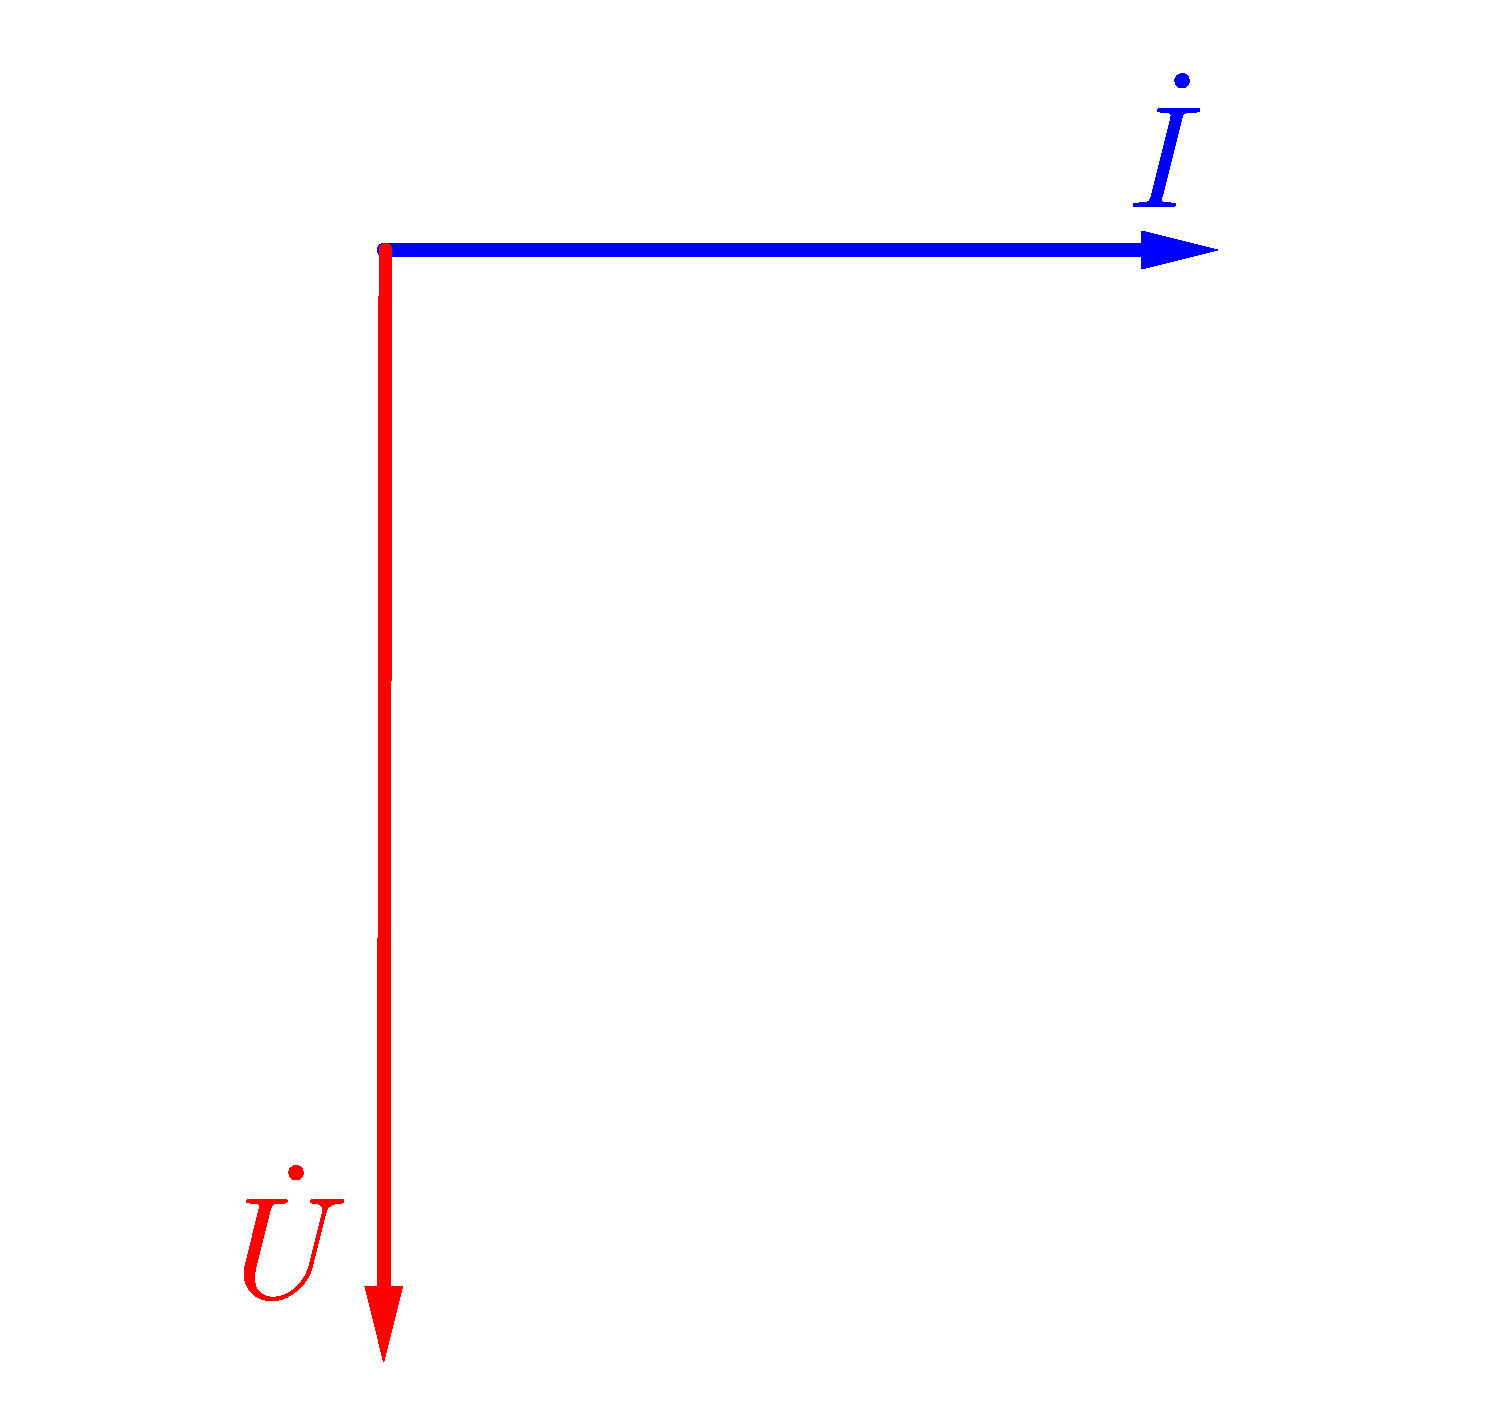
\includegraphics[width=0.65\textwidth]{电容相量图.pdf}
        \caption{电容相量图}
        \label{fig:电容相量图}
        [\kaishu{电压比电流滞后}$90 \degree $]
    \end{minipage}
\end{figure}

事实上,我们也将$j$称作$90 \degree $旋转因子,只要加上了它,就会旋转$90 \degree $.

\begin{table}[htbp]
    \centering
    \caption{单一元件的伏安关系}
    \begin{tblr}{
        row{odd} = {azure8}, 
        row{even} = {gray8},
        colspec={cccc},
        row{1} = {c,2em,azure2,fg=white},
        }
        \diagbox{}{} & 电阻 & 电感 & 电容\\
        电流 & $i=\sqrt{2}I\sin \omega t$ & $i=\sqrt{2}I\sin \omega t$ & $i=\sqrt{2}I\sin \omega t$\\
        电压 & $u=\sqrt{2}IR\sin \omega t$ & $u=\sqrt{2}IX_{\mathrm{L}}\sin \left( \omega t+\frac{\pi}{2} \right) $ & $u=\sqrt{2}IX_{\mathrm{C}}\sin \left( \omega t-\frac{\pi}{2} \right) $\\
        电抗 & $\frac{\dot{U}}{\dot{I}}=R$ & $\frac{\dot{U}}{\dot{I}}=\mathrm{j}X_{\mathrm{L}}$ & $\frac{\dot{U}}{\dot{I}}=-\mathrm{j}X_{\mathrm{C}}$\\
    \end{tblr}
\end{table}

\subsection{\K 单一元件的功率关系}
\Par 首先我们定义:在任意瞬间,电压瞬时值$u$与电流瞬时值$i$的乘积被称为\hl{瞬时功率},即
\begin{equation}
    p=ui
\end{equation}
我们可以写出三种元件的瞬时功率
\begin{align*}
	\text{电阻}p_R&=ui=2I^2R\sin ^2\omega t=I^2R\left( 1-\cos 2\omega t \right)\\
	\text{电感}p_L&=ui=2I^2X_{\mathrm{L}}\sin \omega t\cos \omega t=I^2X_{\mathrm{L}}\sin 2\omega t\\
	\text{电容}p_C&=ui=-2I^2X_{\mathrm{C}}\sin \omega t\cos \omega t=-I^2X_{\mathrm{C}}\sin 2\omega t
\end{align*}
下面我们用{\color{red}红色曲线}代表{\color{red}电压},{\color{blue}蓝色曲线}代表{\color{blue}电流},{\color{green}绿色曲线}代表{\color{green}瞬时功率},作图对比三者之间的差异.
\begin{figure}[htbp]
	\centering
	\begin{minipage}{0.3\textwidth}
        \centering
        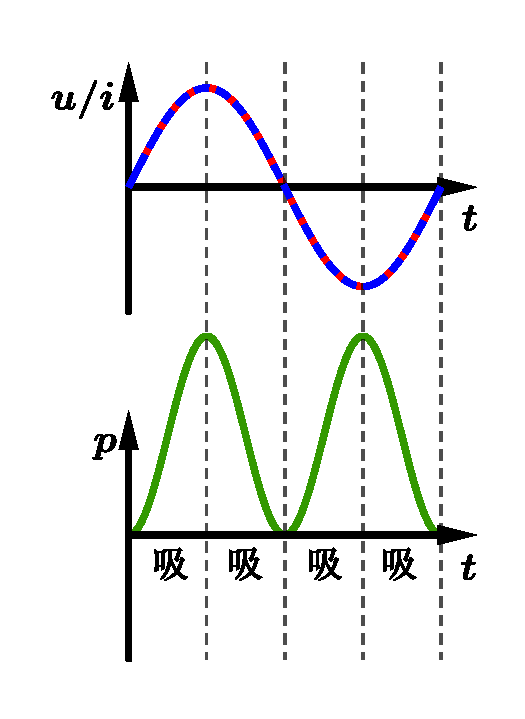
\includegraphics[width=0.95\textwidth]{电阻的瞬时功率.pdf}
        \caption{电阻的瞬时功率}
        \label{fig:电阻的瞬时功率}
    \end{minipage}
    \begin{minipage}{0.3\textwidth}
        \centering
        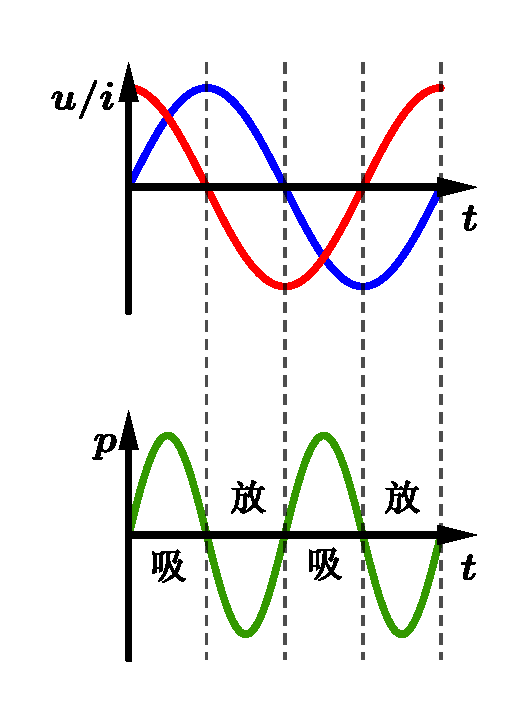
\includegraphics[width=0.95\textwidth]{电感的瞬时功率.pdf}
        \caption{电感的瞬时功率}
        \label{fig:电感的瞬时功率}
    \end{minipage}
    \begin{minipage}{0.3\textwidth}
        \centering
        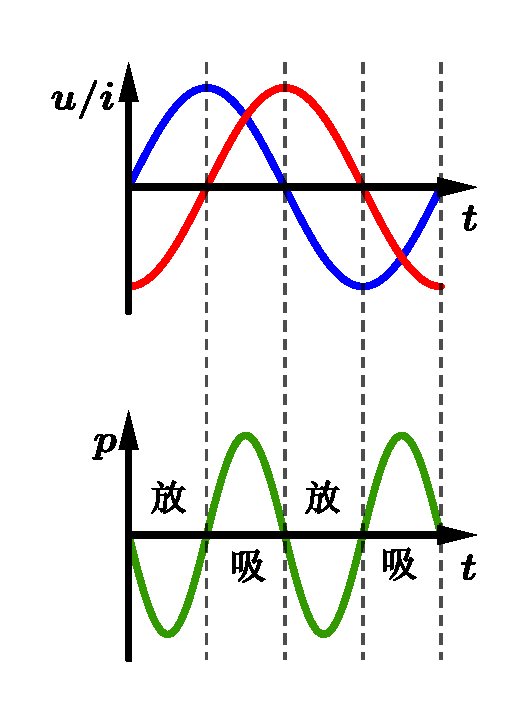
\includegraphics[width=0.95\textwidth]{电容的瞬时功率.pdf}
        \caption{电容的瞬时功率}
        \label{fig:电容的瞬时功率}
    \end{minipage}
\end{figure}

\Par 可以看见,电感和电容在一个周期内的瞬时功率都是有正有负,只有电阻的瞬时功率一直是正,因此我们定义\hl{平均功率}
\begin{equation}
    P=\frac{1}{T}\int_0^T{uidt}
\end{equation}
平均功率又被称作\hl{有功功率}.

\Par 可以知道三种元件的有功功率分别为
\begin{align*}
	\text{电阻}P_R&=\frac{1}{T}\int_0^T{I^2R\left( 1-\cos 2\omega t \right) dt}=I^2RT\\
	\text{电感}P_L&=\frac{1}{T}\int_0^T{I^2X_{\mathrm{L}}\sin \left( 2\omega t \right) dt}=0\\
	\text{电容}P_C&=-\frac{1}{T}\int_0^T{I^2X_{\mathrm{C}}\sin 2\omega tdt}=0
\end{align*}
我们注意到,一个周期内电感和电容的有功功率都是0,为了将它们进行区分,我们定义:电压有效值$U$与电流有效值$I$的乘积,即瞬时功率的幅值
\begin{equation}
    Q=UI
\end{equation}
为\hl{无功功率},其单位为$\mathrm{var}$,读作乏.它表征了储能元件与电源之间能量互换的规模.我们同样写出电感和电容无功功率
\begin{equation*}
    \begin{aligned}
        \text{电感}Q_L&=UI=I^2X_{\mathrm{L}}\\
        \text{电容}Q_C&=UI=-I^2X_{\mathrm{C}}
    \end{aligned}
\end{equation*}


\begin{table}[htbp]
    \centering
    \caption{单一元件的功率关系}
    \begin{tblr}{
        row{odd} = {azure8}, 
        row{even} = {gray8},
        colspec={cccc},
        row{1} = {c,2em,azure2,fg=white}
        }
        \diagbox{}{} & 电阻 & 电感 & 电容\\
        瞬时功率 & $p_R=I^2R\left( 1-\cos 2\omega t \right) $ & $p_L=I^2X_{\mathrm{L}}\sin 2\omega t$ & $p_C=-I^2X_{\mathrm{C}}\sin 2\omega t $\\
        有功功率 & $P_R=I^2RT$ & $P_L= 0$& $P_C= 0$\\
        无功功率 & \diagbox{}{} & $Q_L=I^2X_{\mathrm{L}}$ & $Q_C=-I^2X_{\mathrm{C}}$\\
    \end{tblr}
\end{table}








